\newpage

\section{A Variation of Knoop, Ruthing, and Steffen’s Lazy Code Motion}
\subsection{Where	to	Insert?	}

We want to insert the new computation where it is not partially available there.


\begin{definition}{Anticipable(Very Busy) Expression}
    An	expression	e	is	anticipable	at	a	program	point	p	
    if	e will	be	computed	along	every	path	from	
    p	to	p$_{\mathrm{end}}$,	and	no	 variable	in	e	is	
    redefined	until	its	computation. It	is	safe	to	move	
    an	expression	to	a	basic	block	where	
    that	expression	is	anticipable. By	"safe"	we	mean	
    "performance	safe",	i.e.,	no	extra computation	
    will	be	performed.	Notice	that	if	an	expression	
    e	is	computed	at	a	basic block	where	it	is	both     available
    and	anticipable,	then	that	
    computation	is	clearly	redundant.		

    \begin{figure}[H]
        \centering
         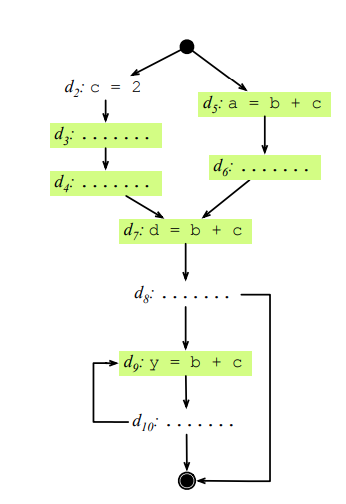
\includegraphics[width=0.5\textwidth]{p89.png}
             \caption{For \texttt{b+c}, the {\color{green}green} blocks are anticipable points. }
             \label{fig:p89}
    \end{figure}
\end{definition}



The key to partial redundancy
elimination is deciding where to add
computations of an expression to
change partial redundancies into full
redundancies (which may then be
optimized away). There	are	now	two	steps	that	we	must	
perform:

\begin{itemize}
\item First,	we	find	the	earliest	places	in	which	
we	can	move	the	computation	of	an	
expression	without	adding	unnecessary	
computations	to	the	CFG.	This	step	is	like	
pushing	the	computation	of	the	
expressions	up.	
\item Second,	we	try	to	move	these	
computations	down,	closer	to	the	places	
where	they	are	necessary,	without	adding	
redundancies	to	the	CFG.	This	phase	is	like	
pulling	these	computations	down	the	CFG. So	that	we	can,	
for	instance,	reduce	register	
pressure.
\end{itemize}

\begin{figure}[H]
    \centering
     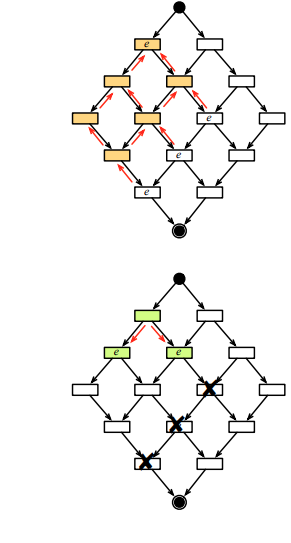
\includegraphics[width=0.3\textwidth]{p90.png}
         \caption{Pushing up, Pulling down.}
         \label{fig:p90}
\end{figure}

\subsubsection{Earliest	Placemen}

We	must	now	find	the	earliest	possible	places	where	we	
can	compute	the	target	expressions.	Earliest	in	the	sense	that	p1	comes	before	p2	if	p1	precedes	
p2	in	any	topological	ordering	of	the	CFG.

\begin{figure}[H]
    \centering
     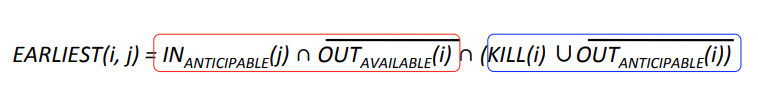
\includegraphics[width=0.6\textwidth]{p91.png}
         
         \label{fig:p91}
\end{figure}


For the {\color{red} Fisrt} part, We	can	move	an	expression	e	to
an	edge	ij	only	if	e	is	anticipabled	at	the	entrance
of	j.	 If	the	expression	is	available	at	the	beginning	of	the	edge,
then	we	should	not	move	it	there.	
But the {\color{blue} Second} part, If	an	expression	is	anticipable	at	i,	
then	we	should	not	move	it	to	ij,	because	we	can	move	it	to	before	i.	
On	the	other	hand,	if	i	kills	the	expression,	then	it	cannot	
be	computed	before	i.


\begin{figure}[H]
    \centering
     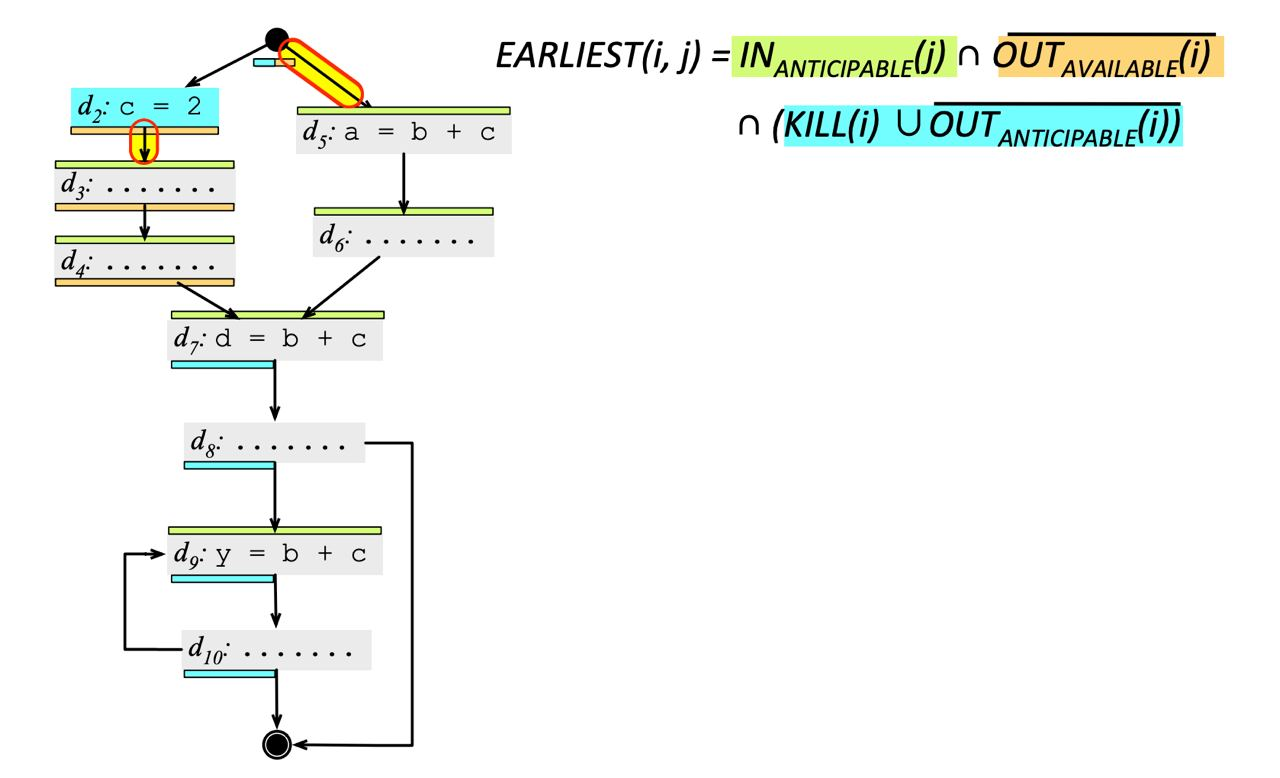
\includegraphics[width=0.8\textwidth]{p92.jpg}
         \caption{An example for calculating EARLIEST.}
         \label{fig:p92}
\end{figure}

\subsubsection{Latest	Placement}


$$
\begin{aligned}
&\operatorname{IN}_{\text {LATER }}(j)=\cap_{i \in \operatorname{pred}(j)} \operatorname{LATER}(i, j) \\
&\operatorname{LATER}(i, j)=\operatorname{EARLIEST}(i, j) \cup\left(\operatorname{IN}_{\text {LATER }}(i) \cap \overline{\operatorname{EXPR}(i)}\right). \\
&
\end{aligned}
$$


LATER(i,j)	is	true	if	we	can	move	the	computation	of	the	
expression	down	the	edge	ij.	 An	expression	e	is	in	
EXPR(i)	if	e	is	computed	at	i.	This	predicate	is	also
 computed	for	edges,	although	we	
have	IN$_\mathrm{LATER}$	being	computed	for	nodes.	



% $$
% \operatorname{LATER}(i, j)=\operatorname{EARLIEST}(i, j) \cup\left(\operatorname{IN}_{\text {LATER }}(i) \cap \overline{\operatorname{EXPR}(i)}\right). 
% $$

For \( \mathrm{LATER}(i,j) \): If	EARLIEST(i,	j)	is	true,	
then	\( \mathrm{LATER}(i,j) \)	is	also	true,	as	we	
can	move	the	computation	of	e	to	edge	ij	without	
causing	redundant	computations. 	If	\( IN_{\mathrm{LATER}}(i,j) \)	is	true,	
and	the	expression	is	not	used	at	i,	
then	LATER(i,j)	is	true.	If	the	expression	is	used	at	i,	then	there	is	no	point	in	
computing	it	at	ij,	because	it	will	be	recomputed	at	i
anyway.	


For \( IN_{\mathrm{LATER}}(i,j) \), it is	a	condition	that	
we	propagate	down.	If	all	the	predecessors	of	a	
node	j	accept	the	
expression	as	nonredundant,	then	we	can	
compute	the	expression	
down	on	j.	

\begin{figure}[H]
    \centering
    \begin{subfigure}{0.3\textwidth}
    \centering
        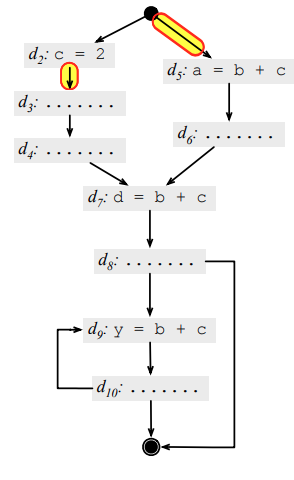
\includegraphics[width=\textwidth]{p94.png}
        \caption{For \texttt{b+c}, 	two	
        earliest	placement	
        points is colored in red.}
        \label{fig:p94}
    \end{subfigure}
    \begin{subfigure}{0.4\textwidth}
    \centering
        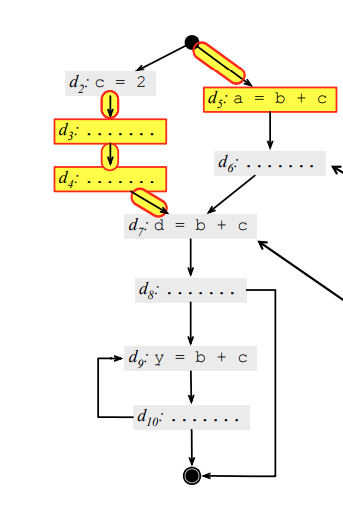
\includegraphics[width=\textwidth]{p95.png}
        \caption{For \texttt{b+c}, Latest placement edhes and blocks.}
        \label{fig:p95}
    \end{subfigure}
    
    \caption{A more complex example of strength reduction.}
       \label{fig:p74-76}
\end{figure}



\subsubsection{Where	to	Insert	Computations?}

We	insert	the	new	computations	at	the	latest	possible	
place.That is 

\begin{figure}[H]
    \centering
     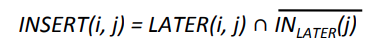
\includegraphics[width=0.6\textwidth]{p96.png}
         
         \label{fig:p96}
\end{figure}


There	are	different	insertion	points,	depending	on	the	
structure	of	the	CFG,	if	x $\in$ INSERT(i,	j):	

\begin{figure}[H]
    \centering
     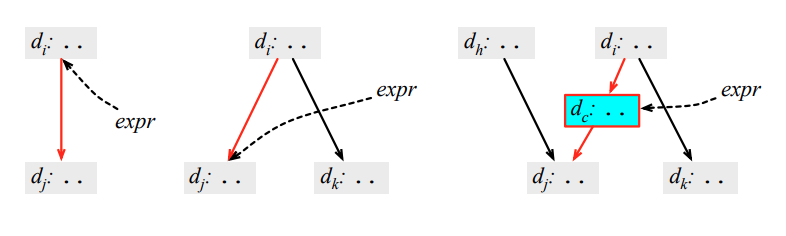
\includegraphics[width=0.6\textwidth]{p97.png}
         \caption{	Different	inser9on	points}
         \label{fig:p97}
\end{figure}
\subsection{Modify CFG}

Rename all compuation of the expression.  

\begin{figure}[H]
    \centering
     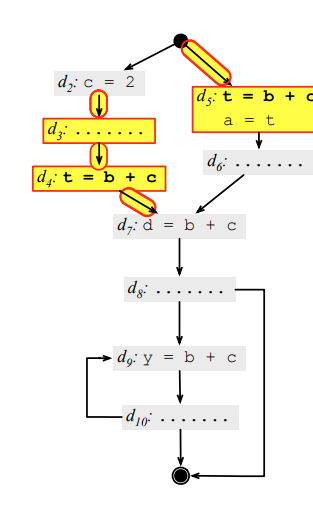
\includegraphics[width=0.4\textwidth]{p100.png}
         \caption{For \texttt{b+c}, the result of applyiny modifying CFG.}
         \label{fig:p100}
\end{figure}


\subsection{Which	Computations	to	Remove?	}
We	remove	computations	that	are	already	covered	by	
the	latest	points,	and	that	we	cannot	use	later	on.	

\begin{figure}[H]
    \centering
     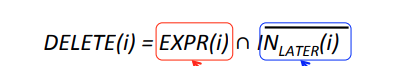
\includegraphics[width=0.6\textwidth]{p98.png}
         
         \label{fig:p98}
\end{figure}




For {\color{red} First} part, of	course,	the	expression	
must	be	used	in	the	block,	
otherwise	we	would	have	
nothing	to	delete. For {\color{blue} second} part, The	expression	may	not	be	a	
computation	that	is	necessary	
later	on.	


\begin{figure}[H]
    \centering
     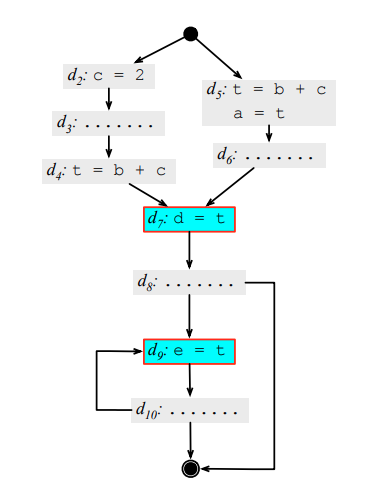
\includegraphics[width=0.4\textwidth]{p101.png}
         \caption{For \texttt{b+c}, the result of applyiny deleting redundancy \texttt{b+c}}
         \label{fig:p100}
\end{figure}



\subsection{A fully explained example}
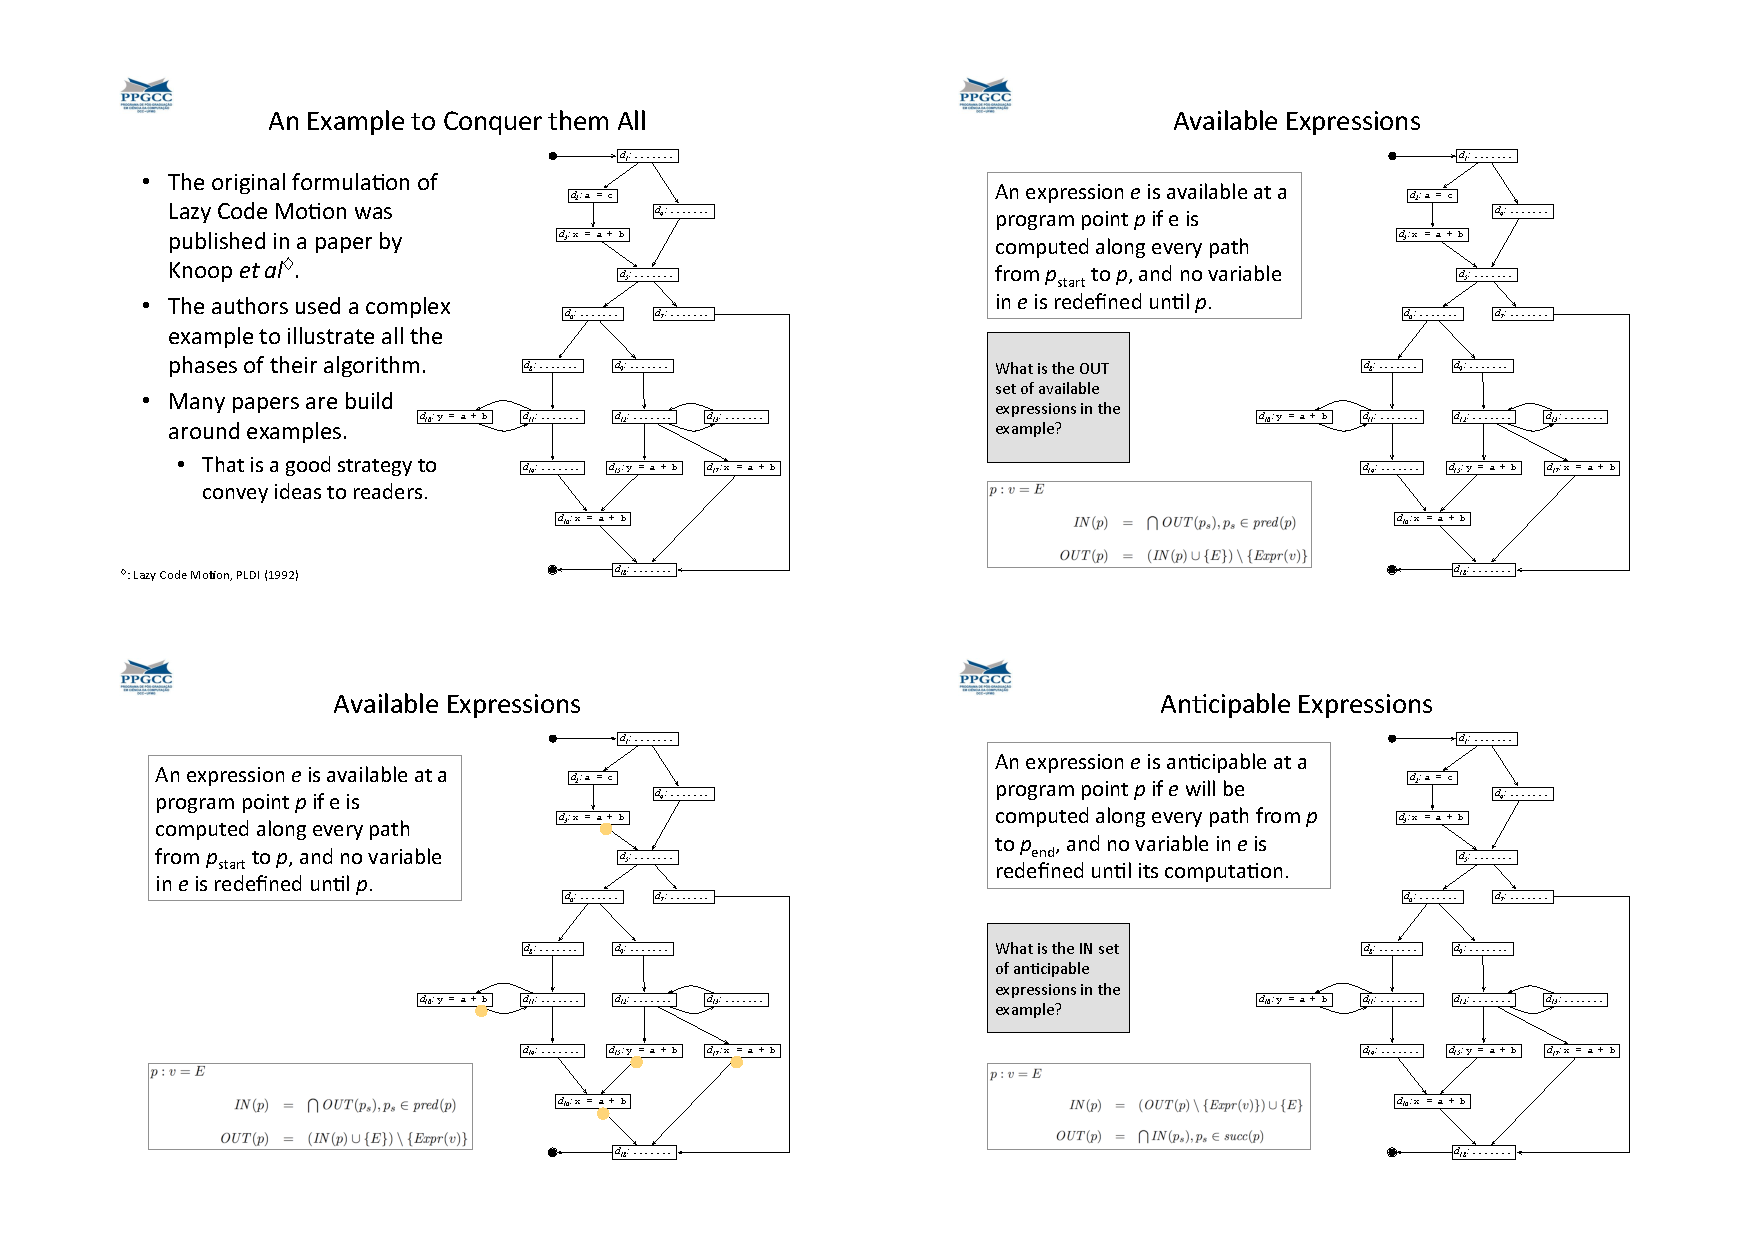
\includepdf[pages={1-}]{p99.pdf}
